\section{Desarrollo}
	\subsection {Tecnologías y Software empleados}
	\begin{itemize}
		\item IntelliJ IDEA 2023.1.2 (Ultimate Editon)
		\item Java correto-17 versión 17.0.17)
		\item Git versión 2.34.1
		\item MySQL Workbench 8 versión 8.0.32
		\item Mysql Ver 8.0.33-0ubuntu0.22.04.2
		\item Spring Boot 3.0.1
		\item Ubuntu 22.04 LTS
		\item Postman v10.15.1
	\end{itemize}
	\subsection{Procedimiento}
	Desde un requerimiento general se debe realizar un análisis a profundidad sobre las necesidades, dicho análisis debe ser genérico; es decir debe valer para cualquier aplicación que requiera de esa funcionalidad.\\
	
	Una vez teniendo el análisis se revisa la documentación de Spring Boot sobre la implementación de los microservicios, con esto podemos transportar el análisis realizado en papel a código de programación, en este caso utilizamos Java como lenguaje de programación principal apoyándonos de un framework que facilita la implementación de funcionalidades que son demandantes de tiempo al estar desarrollando como lo es la conexión a base de datos, facilidad en integrar dependencias, facilidad de visualizar el desarrollo en el navegador integrando un contenedor de aplicaciones web para ser desplegado.
	
	\subsubsection{Patrón MVC}
	Utilizamos el patrón de desarrollo MVC para logar la estructura de carpetas ordenadas sin mezclar la lógica de negocio con la funcionalidad a implementar. El patrón de desarrollo MVC se compone de esta estructura:
	\begin{itemize}
		\item Modelos: Representan los datos y la lógica de negocio de la aplicación, con ellas gestionamos las entidades de las bases de datos, validaciones a nivel de tipo de datos y limitantes de aceptación.
		En estos componentes es donde se establece la cardinalidad de las entidades a utilizar.
		\item Vista: Es la interfaz de usuario de la aplicación, se encarga de la representación visual de los datos y la interacción con el usuario, en este caso omitimos esta parte en microservicios ya que estos solo devuelven colecciones de tipo Json o xml según sean las necesidades de la aplicación a escalar.
		\item Controlador: Actuá como intermediario entre el modelo y la vista, además su parte principal es controlar el flujo de la aplicación, coordinando las diferentes acciones y actualizaciones internas del sistema.
	\end{itemize}
	\begin{minipage}{0.3\textwidth}
		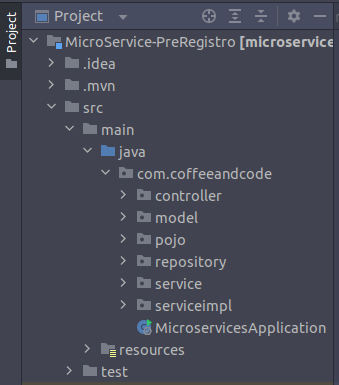
\includegraphics[width=\linewidth]{img/mvc.png}
	\end{minipage}
	\hfill
	\begin{minipage}{0.7\textwidth}
		Se decide utilizar este patrón de desarrollo, debido a que permite la modularidad y flexibilidad en el desarrollo de nuestro microservicio, cada componente tiene una responsabilidad especifica y se puede modificar o remplazar de manera independiente, la ejemplificación del patrón MVC la podemos observar en la siguiente imagen.
	\end{minipage}
	
	\subsubsection{Servicios, interfaces de repositorios, implementación de interfaces.}
	Una de las facilidades que permite Spring Boot es la inyección de dependencias, con estas se hace referencia a los servicios e interfaces de repositorios, en otros componentes, esto similar al funcionamiento de los controladores.\\
	Se utilizan para dividir las responsabilidades y facilitar la prueba y mantenimiento del código, se podría decir que también son pieza importante donde se permite la modularidad, escalabilidad y flexibilidad del sistema.
	\begin{itemize}
		\item Servicios: Aquí se implementa la lógica de negocio de una aplicación, representan la capa intermedia entre los controladores y los repositorios, con ellas se busca proporcionar funcionalidad especifica y operaciones más complejas.
		\item Interfaces de repositorios: Definen métodos para interactuar con la capa de almacenamiento de datos(bases de datos, o servicios web). Permiten la abstracción de la lógica de acceso a datos y proporcionan una forma estandarizada para las operaciones CRUD(Crear, Leer, Actualizar, Eliminar) sobre los objetos persistentes. 
		\item Implementación de interfaces: Contienen la creación de clases que implementan las interfaces definidas, dichas clases contienen la lógica concreta para llevar a cabo las operaciones definidas en las interfaces, es decir aquí es en donde se desarrolla el método completo.
	\end{itemize}
	
	
	
	\subsubsection{Desarrollo de microservicios}
	Iniciamos con el proceso de desarrollo de microservicios, primero definimos que tipo de datos aceptará y entregará nuestro microservicio, para este caso especifico se decide que será en Json.\\
	
	Utilizando MVC definimos las entidades de nuestra base de datos en el apartado \textbf{model}, en este se establece la cardinalidad que hemos definido en nuestro diagrama entidad relación que diseñamos durante el análisis de requerimientos, es aquí donde definimos los atributos que contendrá la tabla, ademas del nombre de la misma todo con notaciones que pertenecen a dependencias utilizadas para \textbf{maven} apoyados del framework \textbf{Spring Boot.}\\
	
	Utilizamos los controladores para poder manipular las re-direcciones dentro de nuestro sistema, ademas esta es la capa donde definimos métodos de entrada y salida de datos, es decir por aquí ingresan las peticiones y retornamos las respuestas, también en este apartado es en donde inyectamos las dependencias InterfaceXXXXXService, dichas dependencias proveen los métodos para traer o insertar información a nuestra base de datos.\\
	
	Utilizamos la implementación los servicios para poder comunicarnos con el repositorio, así podemos tener acceso a base de datos, definimos métodos como son listar, crear, actualizar, búsqueda por x campo.
	Dichos métodos serán bien desarrollados en ImplxxxxxxxService y serán consumidos en el controlador para brindar funcionalidad a nuestro microservicio.
	\begin{lstlisting}[style=JavaStyle, caption=Ejemplo de definición de interfacexxxxxxService, label=lst:java]
		package com.coffeeandcode.service;
		
		import com.coffeeandcode.model.AcademicDataModel;
		
		import java.util.List;
		import java.util.Optional;
		
		public interface InterfaceAcademicDataService {
			public List<AcademicDataModel> listallAcademicDatas();
			
			public Optional<AcademicDataModel> getAcademicDataById(int idAcademicData);
			
			public AcademicDataModel createAcademicData(AcademicDataModel academicDatamodel);
			
			public AcademicDataModel saveAcademicData(AcademicDataModel academicDatamodel);
			
			public AcademicDataModel updateAcademicData(int idAcademicData, AcademicDataModel academicDatamodel);
			
			public boolean deleteAcademicData(int idAcademicData);
		}
	\end{lstlisting}
	
	\subsubsection{Prueba de funcionamiento con Postman}
	Para probar la funcionalidad de nuestro servicios, existen dos maneras, una es con un software llenado \textbf{Postman} y la otra es desde la terminal de nuestro sistema, donde estemos trabajando.\\
	En esta ocasión probaremos con Postman debido a la facilidad que nos provee, antes cabe mencionar que los métodos están desarrollados en el controlador, dichos metodos reciben json y devuelven json, el contenido es definido por la logia implementada.
	\begin{lstlisting}[style=JavaStyle, caption=Ejemplo de metodos desarrollados del lado del controlador, label=lst:java]
		public class PersonalDataController {
		private final InterfacePersonalDataService interfacePersonalDataService;
		
		@Autowired
		public PersonalDataController(InterfacePersonalDataService interfacePersonalDataService) {
			this.interfacePersonalDataService = interfacePersonalDataService;
		}
		
		@PostMapping("/save")
		public ResponseEntity<Object> createPersonalData(@RequestBody PersonalDataModel personalData)...
		
		@GetMapping("/list")
		public ResponseEntity<Object> index()...
	
		@PutMapping("/update/{id}")
		public ResponseEntity<Object> updatePersonalData(@PathVariable int id, @RequestBody PersonalDataModel personalData)...
		
		@DeleteMapping("/delete/{id}")
		public ResponseEntity<String> deletePersonalData(@PathVariable int id)...
		
		@GetMapping("/search/{id}")
		public ResponseEntity<Object> getPersonalData(@PathVariable int id)
	
		}
	\end{lstlisting}
	Se omite el desarrollo debido a que algunos métodos son demasiados largos para mostrarlos, procederemos a explicar el funcionamiento breve de cada uno de los métodos.
	\begin{itemize}
		\item createPersonalData: Nos permite ingresar un json con una estructura especifica y mediante interfacePersonalDataService podremos agregar los datos contenidos en el json a la base de datos, dicho método nos devuelve el json del elemento que se agrega, si por alguna cuestión no es posible agregar nos devuelve un mensaje de error diciendo que no fue posible el almacenamiento.
		\item index: ejecuta una consulta en la cual nos regresa todos los datos contenidos en la base de datos. 
		\item updatePersonalData: Este método a razón de un id nos permite actualizar el contenido directamente de la base de datos del elemento deseado.
		\item deletePersonalData: Nos permite eliminar un elemento a razón de recibir el id de dicho elemento.
		\item getPersonalData: Nos devuelve un objeto especifico, lo pediremos a razón del id proporcionado.
	\end{itemize}

	Dichos métodos anteriormente explicados se pueden combinar entre si para proveer de más funcionalidades a nuestro microservicio, si alguna consulta no hace lo que se requiere y se pretende ser las especifico podemos definir una consulta nativa de SQL en el repositorio correspondiente.
%\subsection{Resultados}
%Aquí describir los resultados obtenidos evidencia del programa funcionando y describir las funcionalidades puedes incluir imágenes.